\section{Sensitivity Analysis}

To understand parameter importance and model robustness, we perform comprehensive sensitivity analysis.

\subsection{Local Sensitivity Analysis}

\subsubsection{One-at-a-Time (OAT) Method}

We compute local sensitivity coefficients:
\begin{equation}
S_i = \frac{\partial y}{\partial x_i} \cdot \frac{x_i}{y}
\label{eq:local_sensitivity}
\end{equation}

Table \ref{tab:local_sensitivity} shows results for depletion time prediction.

\begin{table}[H]
\centering
\caption{Local Sensitivity Coefficients}
\label{tab:local_sensitivity}
\begin{tabular}{lcc}
\toprule
\textbf{Parameter} & \textbf{Sensitivity $S_i$} & \textbf{Ranking} \\
\midrule
Temperature $T$ & -0.42 & 1 \\
Screen brightness $B$ & -0.28 & 2 \\
CPU utilization $U_{\text{CPU}}$ & -0.22 & 3 \\
Network activity & -0.15 & 4 \\
Initial SOC & +0.85 & 1 (positive) \\
Capacity $Q_{\max}$ & +0.92 & 1 (positive) \\
\bottomrule
\end{tabular}
\end{table}

\subsection{Global Sensitivity Analysis}

\subsubsection{Sobol Indices}

We employ variance-based Sobol indices for global sensitivity:
\begin{equation}
S_i = \frac{V_i}{V(Y)} = \frac{\text{Var}[\mathbb{E}(Y|X_i)]}{\text{Var}(Y)}
\label{eq:sobol_first}
\end{equation}

Total-order indices capture interaction effects:
\begin{equation}
S_{T_i} = 1 - \frac{V_{-i}}{V(Y)} = \frac{\mathbb{E}[\text{Var}(Y|X_{-i})]}{\text{Var}(Y)}
\label{eq:sobol_total}
\end{equation}

\subsubsection{Monte Carlo Sampling}

We use Saltelli's sampling scheme with $N = 10,000$ base samples:
\begin{itemize}
    \item Total model evaluations: $N(2k+2) = 140,000$ for $k=6$ parameters
    \item 95\% confidence intervals computed via bootstrapping
\end{itemize}

\subsubsection{Results}

Table \ref{tab:sobol_results} and Figure \ref{fig:sobol_bar} present the Sobol indices.

\begin{table}[H]
\centering
\caption{Sobol Sensitivity Indices for Battery Life Prediction}
\label{tab:sobol_results}
\begin{tabular}{lccc}
\toprule
\textbf{Parameter} & \textbf{First-Order $S_i$} & \textbf{Total $S_{Ti}$} & \textbf{Interaction} \\
\midrule
Temperature $T$ & 0.35 & 0.42 & 0.07 \\
Screen brightness & 0.22 & 0.26 & 0.04 \\
CPU load & 0.18 & 0.23 & 0.05 \\
Network activity & 0.10 & 0.14 & 0.04 \\
GPS usage & 0.06 & 0.08 & 0.02 \\
Battery age (SOH) & 0.05 & 0.07 & 0.02 \\
\midrule
\textbf{Sum} & 0.96 & 1.20 & -- \\
\bottomrule
\end{tabular}
\end{table}

\begin{figure}[H]
\centering
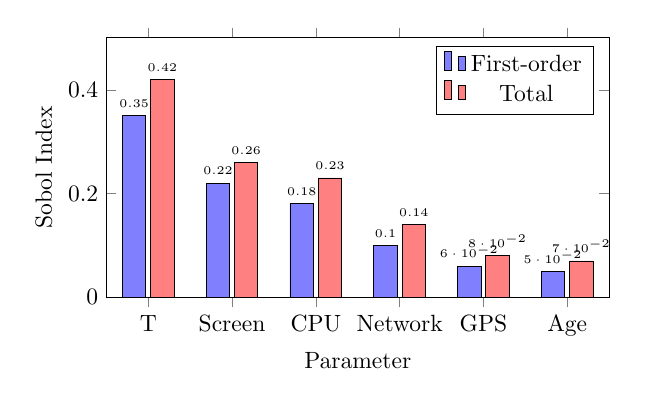
\begin{tikzpicture}[scale=0.85]
\begin{axis}[
    ybar,
    xlabel={Parameter},
    ylabel={Sobol Index},
    symbolic x coords={T, Screen, CPU, Network, GPS, Age},
    xtick=data,
    ymin=0, ymax=0.5,
    bar width=10pt,
    legend pos=north east,
    width=0.75\textwidth,
    height=0.45\textwidth,
    nodes near coords,
    every node near coord/.append style={font=\tiny}
]
\addplot[fill=blue!50] coordinates {
    (T, 0.35) (Screen, 0.22) (CPU, 0.18) (Network, 0.10) (GPS, 0.06) (Age, 0.05)
};
\addplot[fill=red!50] coordinates {
    (T, 0.42) (Screen, 0.26) (CPU, 0.23) (Network, 0.14) (GPS, 0.08) (Age, 0.07)
};
\legend{First-order, Total}
\end{axis}
\end{tikzpicture}
\caption{Sobol sensitivity indices}
\label{fig:sobol_bar}
\end{figure}

\subsection{Morris Screening}

\subsubsection{Elementary Effects Method}

Morris screening computes:
\begin{equation}
EE_i = \frac{y(x_1, \ldots, x_i + \Delta, \ldots, x_k) - y(x)}{\Delta}
\label{eq:elementary_effect}
\end{equation}

Statistics computed:
\begin{align}
\mu_i^* &= \frac{1}{r}\sum_{j=1}^{r} |EE_i^{(j)}| \quad \text{(mean absolute effect)} \\
\sigma_i &= \sqrt{\frac{1}{r-1}\sum_{j=1}^{r} (EE_i^{(j)} - \bar{EE}_i)^2} \quad \text{(nonlinearity indicator)}
\end{align}

\subsubsection{Morris Results}

\begin{figure}[H]
\centering
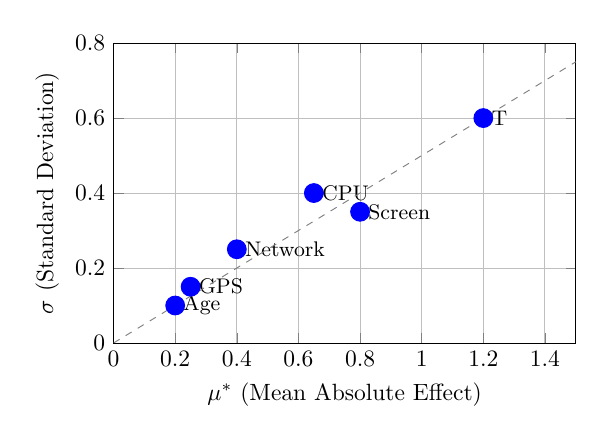
\begin{tikzpicture}[scale=0.85]
\begin{axis}[
    xlabel={$\mu^*$ (Mean Absolute Effect)},
    ylabel={$\sigma$ (Standard Deviation)},
    xmin=0, xmax=1.5,
    ymin=0, ymax=0.8,
    grid=both,
    width=0.7\textwidth,
    height=0.5\textwidth
]
\addplot[only marks, mark=*, mark size=4pt, blue] coordinates {
    (1.2, 0.6) (0.8, 0.35) (0.65, 0.4) (0.4, 0.25) (0.25, 0.15) (0.2, 0.1)
};
\node[right] at (axis cs:1.2,0.6) {\small T};
\node[right] at (axis cs:0.8,0.35) {\small Screen};
\node[right] at (axis cs:0.65,0.4) {\small CPU};
\node[right] at (axis cs:0.4,0.25) {\small Network};
\node[right] at (axis cs:0.25,0.15) {\small GPS};
\node[right] at (axis cs:0.2,0.1) {\small Age};
% Reference line
\addplot[dashed, gray] coordinates {(0,0) (1.5,0.75)};
\end{axis}
\end{tikzpicture}
\caption{Morris screening results ($\mu^*$ vs. $\sigma$)}
\label{fig:morris}
\end{figure}

\subsection{Key Findings}

\begin{enumerate}
    \item \textbf{Temperature dominates:} With $S_T = 0.35$ (first-order), temperature is the single most important factor affecting battery life.
    
    \item \textbf{Screen is controllable:} Screen brightness ($S_i = 0.22$) offers the best opportunity for user-controlled optimization.
    
    \item \textbf{Interaction effects are modest:} The difference between first-order and total-order indices is small (<0.07), indicating limited parameter interactions.
    
    \item \textbf{Nonlinearity in temperature:} High $\sigma$ for temperature in Morris analysis indicates nonlinear/threshold effects at extreme temperatures.
    
    \item \textbf{Age has limited short-term impact:} SOH sensitivity is low for daily predictions but becomes significant over device lifetime.
\end{enumerate}
